\let\negmpace\undefined
\let\negthickspace\undefined
\documentclass[journal]{IEEEtran}
\usepackage[a5paper, margin=10mm, onecolumn]{geometry}
\usepackage{tfrupee} % Include tfrupee package
\setlength{\headheight}{1cm} % Set the height of the header box
\setlength{\headsep}{0mm}     % Set the distance between the header box and the top of the text
\usepackage{gvv-book}
\usepackage{gvv}
\usepackage{cite}
\usepackage{amsmath,amssymb,amsfonts,amsthm}
\usepackage{algorithmic}
\usepackage{graphicx}
\usepackage{textcomp}
\usepackage{xcolor}
\usepackage{txfonts}
\usepackage{listings}
\usepackage{enumitem}
\usepackage{mathtools}
\usepackage{gensymb}
\usepackage{comment}
\usepackage[breaklinks=true]{hyperref}
\usepackage{tkz-euclide} 
\usepackage{listings}
\def\inputGnumericTable{}                                 
\usepackage[latin1]{inputenc}                                
\usepackage{color}                                            
\usepackage{array}                                            
\usepackage{longtable}                                       
\usepackage{calc}                                             
\usepackage{multirow}                                         
\usepackage{hhline}                                           
\usepackage{ifthen}                                           
\usepackage{lscape}
\renewcommand{\thefigure}{\theenumi}
\renewcommand{\thetable}{\theenumi}
\setlength{\intextsep}{10pt} % Space between text and floats


\renewcommand{\thetable}{\theenumi}
\begin{document}
\bibliographystyle{IEEEtran}
\title{Question-9-9.3-25}
\author{EE24BTECH11035 - KOTHAPALLI AKHIL}
{\let\newpage\relax\maketitle}
\vspace{-10mm}
\textbf{Question}:\\
Using the method of integration, find the area of the region bounded by the lines
$3x-2y+1=0$, $2x+3y-21=0$and $x-5y+9=0$.\\
\textbf{Solution};\\
   The lines Given are :\\
   $3x-2y+1=0$, $2x+3y-21=0$and $x-5y+9=0$\\
   The general form of line equation in matrix form is $h^T+m=0$\\
   Writing the Given lines in the form of matrices ,
   \begin{equation}
     h_1^T+m_1=0 \quad  where\quad  h_1=\myvec{3\\-2} , x=\myvec{x\\y} , m_1=1  
   \end{equation}
   \begin{equation}
         h_2^T+m_2=0\quad   where \quad  h_2=\myvec{2\\3} , m_2=-21 
   \end{equation}
   \begin{equation}
        h_3^T+m_3=0  \quad where\quad  h_3=\myvec{1\\-5} , m_3=9 
   \end{equation}
   Solving The Line equations to get points of intersections ,\\
   By Solving First two equations, We get point of intersection as ,
   \begin{equation}
       P_1=\myvec{\frac{36}{13} \\ \frac{121}{26}}
   \end{equation}
Similarly, 
\begin{equation}
     P_2=\myvec{6\\3} ,
     P_3=\myvec{1\\2}
\end{equation}
We now calculate the area of the region using integration. The area is the integral of the top function minus the bottom function over the interval.\\
Equation for the Line Between $P_1$ and $P_2$:
The slope of the line between $P_1$ and $P_2$ is:
\begin{equation}
m_1 = \frac{3 - \frac{121}{26}}{6 - \frac{36}{13}} = -\frac{43}{52}
\end{equation}

The equation of the line is:
\begin{equation}
y - 3 = -\frac{43}{52}(x - 6)
\end{equation}

Equation for the Line Between $P_2$ and $P_3$:\\
The slope of the line between $P_2$ and $P_3$ is:
\begin{equation}
m_2 = \frac{2 - 3}{1 - 6} = \frac{1}{5}
\end{equation}

The equation of the line is:
\begin{equation}
y - 3 = \frac{1}{5}(x - 6)
\end{equation}

Equation for the Line Between $P_3$ and $P_1$:
The slope of the line between $P_3$ and $P_1$ is:
\begin{equation}
m_3 = \frac{\frac{121}{26} - 2}{\frac{36}{13} - 1} = \frac{69}{52}
\end{equation}

The equation of the line is:
\begin{equation}
y - 2 = \frac{69}{52}(x - 1)
\end{equation}
We now calculate the area using the definite integral:
\begin{equation}
A = \int_{x_1}^{x_2} \left( f(x) - g(x) \right) \, dx
\end{equation}
\begin{equation}
A = \int_{1}^{6} \left( \left( -\frac{43}{52}(x - 6) + 3 \right) - \left( \frac{1}{5}(x - 6) + 3 \right) \right) dx
\end{equation}

\begin{equation}
A = \int_{1}^{6} \left( -\frac{43}{52}x + \frac{43 \cdot 6}{52} - \frac{1}{5}x + \frac{6}{5} \right) dx
\end{equation}
\begin{equation}
A = \left[ -\frac{43}{104}x^2 + \frac{43 \cdot 6}{52}x - \frac{1}{10}x^2 + \frac{6}{5}x \right]_{1}^{6}
\end{equation}

After evaluating the integral, we find the area is:
\begin{equation}
A = 6.5 \, \text{square units}
\end{equation}

Thus, the area of the region bounded by the lines is 6.5 square units.
\begin{figure}[h!]
	\centering
	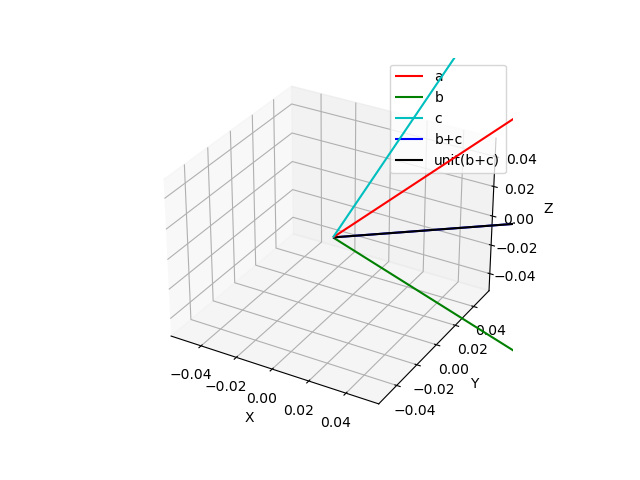
\includegraphics[width=0.5\linewidth]{figs/Figure_1.png}
	\caption{Area enclosed between the 3 Lines}
	\label{stemplot}
\end{figure}	
\end{document}


